% !TeX program = xelatex
% !TeX encoding = UTF-8
% !TeX TXS-program:compile = txs:///xelatex | txs:///xelatex
\documentclass[aspectratio=169, table, 12pt]{beamer}

% Preamble bersama seluruh slide mata kuliah ini.
% Dipanggil dari slides/sessionXX/sessionXX.tex tepat sesudah baris
% \documentclass[aspectratio=169, table, 12pt]{beamer}
% Paket tambahan yang hanya dibutuhkan satu sesi ditulis di berkas sesi itu.

\usepackage{colortbl}
\usepackage{xcolor}
\usepackage{listings}
\usepackage{tabularx}
\usepackage{booktabs}
\usepackage{tikz}
\usepackage{pgfplots}
\usepackage{fontspec}
\usepackage[english,bahasai]{babel}
\pgfplotsset{compat=1.18}
\usetikzlibrary{arrows.meta, positioning, calc, fit, shapes.geometric,
  shapes.multipart, backgrounds, matrix, chains, trees}

\makeatletter
\def\input@path{{../theme/}}
\makeatother
\graphicspath{{../theme/}{../../figures/}}
% Stub symlink Windows memakai tema cadangan sampai aset institusi tersedia.
\IfFileExists{../theme/beamerthemePradita.sty}{%
  \usetheme{Pradita}
}{%
  \usetheme{Madrid}
  \setmainfont{TeX Gyre Heros}
  \setsansfont{TeX Gyre Heros}
  \setbeamertemplate{navigation symbols}{}
}

\definecolor{praditagreen}{RGB}{37, 113, 71}
\setbeamercolor{structure}{fg=praditagreen}
\setbeamercolor{palette primary}{bg=praditagreen,fg=white}
\setbeamercolor{palette secondary}{bg=praditagreen!80!black,fg=white}
\setbeamercolor{palette tertiary}{bg=praditagreen!60!black,fg=white}
\setbeamerfont{frametitle}{size=\large}
\setbeamertemplate{caption}[numbered]

% Ukuran header mengikuti teks agar judul panjang tidak menabrak logo.
\setbeamercolor{frametitle}{bg=white,fg=black}
\setbeamertemplate{frametitle}{%
  \begin{beamercolorbox}[wd=\paperwidth,sep=0.2cm]{frametitle}
    \begin{minipage}[c]{0.77\paperwidth}
      \raggedright\fontsize{16}{18}\selectfont\bfseries\insertframetitle
      \ifx\insertframesubtitle\empty\else
        \par\small\mdseries\insertframesubtitle
      \fi
    \end{minipage}\hfill
    \begin{minipage}[c]{0.15\paperwidth}
      \IfFileExists{../theme/classFiles/logo_universitas.png}{%
        
\includegraphics[width=\linewidth]{../theme/classFiles/logo_universitas.png}%
      }{}
    \end{minipage}
  \end{beamercolorbox}
}
\setbeamertemplate{footline}{%
  \ifnum\value{framenumber}>1
    \begin{beamercolorbox}[wd=\paperwidth,ht=0.35cm,dp=0.15cm,
      leftskip=0.3cm,rightskip=0.3cm]{palette primary}
      \footnotesize\bfseries\insertframenumber/\inserttotalframenumber
      \hfill IT40813
    \end{beamercolorbox}
  \fi
}
\DeclareRobustCommand{\berkas}[1]{\path{#1}}

% Tema membuat garis tabel berwarna putih. Dikembalikan agar tabel terbaca.
\arrayrulecolor{black}
\setlength{\arrayrulewidth}{0.5pt}

\lstdefinelanguage{yaml}{
  basicstyle=\ttfamily\scriptsize,
  keywordstyle=\color{blue}\bfseries,
  commentstyle=\color{gray}\itshape,
  stringstyle=\color{red},
  showstringspaces=false,
  breaklines=true,
  frame=lines,
  numbers=none,
  backgroundcolor=\color{lightgray!10},
  tabsize=2,
  morecomment=[l]{\#}
}

\lstdefinelanguage{json}{
  basicstyle=\ttfamily\scriptsize,
  stringstyle=\color{red},
  commentstyle=\color{gray},
  breaklines=true,
  showstringspaces=false,
  tabsize=2,
  numbers=none,
  frame=lines,
  backgroundcolor=\color{lightgray!10},
  string=[s]{"}{"}
}

\lstdefinelanguage{bash}{
  keywords={},
  basicstyle=\ttfamily\scriptsize,
  ndkeywords={docker, kubectl, helm, curl, git, terraform},
  ndkeywordstyle=\color{purple}\bfseries,
  sensitive=true,
  commentstyle=\color{gray},
  numbers=none,
  breaklines=true,
  frame=lines,
  backgroundcolor=\color{lightgray!10},
  tabsize=2,
  comment=[l]{\#},
  showstringspaces=false
}

\lstdefinelanguage{http}{
  keywords={GET, POST, PUT, PATCH, DELETE, HEAD, OPTIONS, HTTP},
  basicstyle=\ttfamily\scriptsize,
  keywordstyle=\color{blue}\bfseries,
  sensitive=true,
  numbers=none,
  breaklines=true,
  frame=lines,
  backgroundcolor=\color{lightgray!10},
  tabsize=2,
  showstringspaces=false
}

\subtitle{IT40813 · IT Governance, Risk \& Compliance}
\author{\textbf{Alfa Yohannis}}


% Sampul membatasi judul di panel putih tema rujukan Pradita.
\setbeamertemplate{title page}{%
  \begin{tikzpicture}[remember picture,overlay]
    \node[anchor=north west,inner sep=0pt,text width=8.8cm]
      at ([xshift=1cm,yshift=-3.15cm]current page.north west) {%
        {\small\insertsubtitle\par}\vspace{0.25cm}
        \resizebox{8.8cm}{!}{\begin{minipage}{12cm}
          \raggedright\color{praditagreen}\bfseries\inserttitle
        \end{minipage}}
      };
    \node[anchor=south west,inner sep=0pt]
      at ([xshift=1cm,yshift=1.65cm]current page.south west)
      {\small\insertdate};
    \node[anchor=west,inner sep=0pt,text=white]
      at ([xshift=0.8cm,yshift=0.75cm]current page.south west)
      {\small\insertauthor};
  \end{tikzpicture}
}


\title{\Huge COBIT 2019\\ \vspace{10pt} Sistem dan Faktor Desain}
\date{Pertemuan 04}

\begin{document}

\frame{\titlepage}

\begin{frame}
  \frametitle{Isi Pertemuan}
  \vspace{14pt}
  \begin{columns}[t]
    \column{0.5\textwidth}
    {\small\tableofcontents[sections={1-5}]}

    \column{0.5\textwidth}
    {\small\tableofcontents[sections={6-9}]}
  \end{columns}
\end{frame}

\begin{frame}{\hfill}
  \centering
  \Huge{\textbf{Direksi berkata:\\Terapkan COBIT.\\Mulai dari mana?}}
\end{frame}

\section{Tujuan dan Konteks}

\begin{frame}{{\Large Tujuan Pembelajaran}}
  \vspace{10pt}
  \begin{itemize}
    \item Menjelaskan komponen sistem tata kelola dan 40 objektif tata kelola dan manajemen dalam
          COBIT 2019.
    \item Menerapkan faktor desain dan \textit{goals cascade} untuk memilih objektif yang paling
          penting bagi sebuah organisasi.
    \item Menilai tingkat kapabilitas saat ini untuk objektif prioritas berdasarkan bukti, bukan
          pengakuan.
  \end{itemize}
\end{frame}

\begin{frame}{{\Large Masalah: Perintah Tanpa Masalah yang Jelas}}
  \vspace{6pt}
  \small
  \begin{itemize}
    \item Misalkan audit menemukan 6 dari 30 akun vendor masih aktif setelah penugasan berakhir.
    \item Direktur utama berkata ``Terapkan COBIT''. Kepala TI membuka daftar 40 objektif.
    \item Konsultan menawarkan penilaian semua objektif dengan satu angka rata-rata.
    \item Direktur pelayanan bertanya apakah angka itu memperpendek antrean. Tidak ada jawaban.
    \item Kerangka diperlakukan sebagai daftar pekerjaan seragam. Prosedur bertambah, akun vendor
          tetap tidak ditinjau.
  \end{itemize}
\end{frame}

\begin{frame}{{\Large Diagram Konsep Bab 4}}
  \centering
  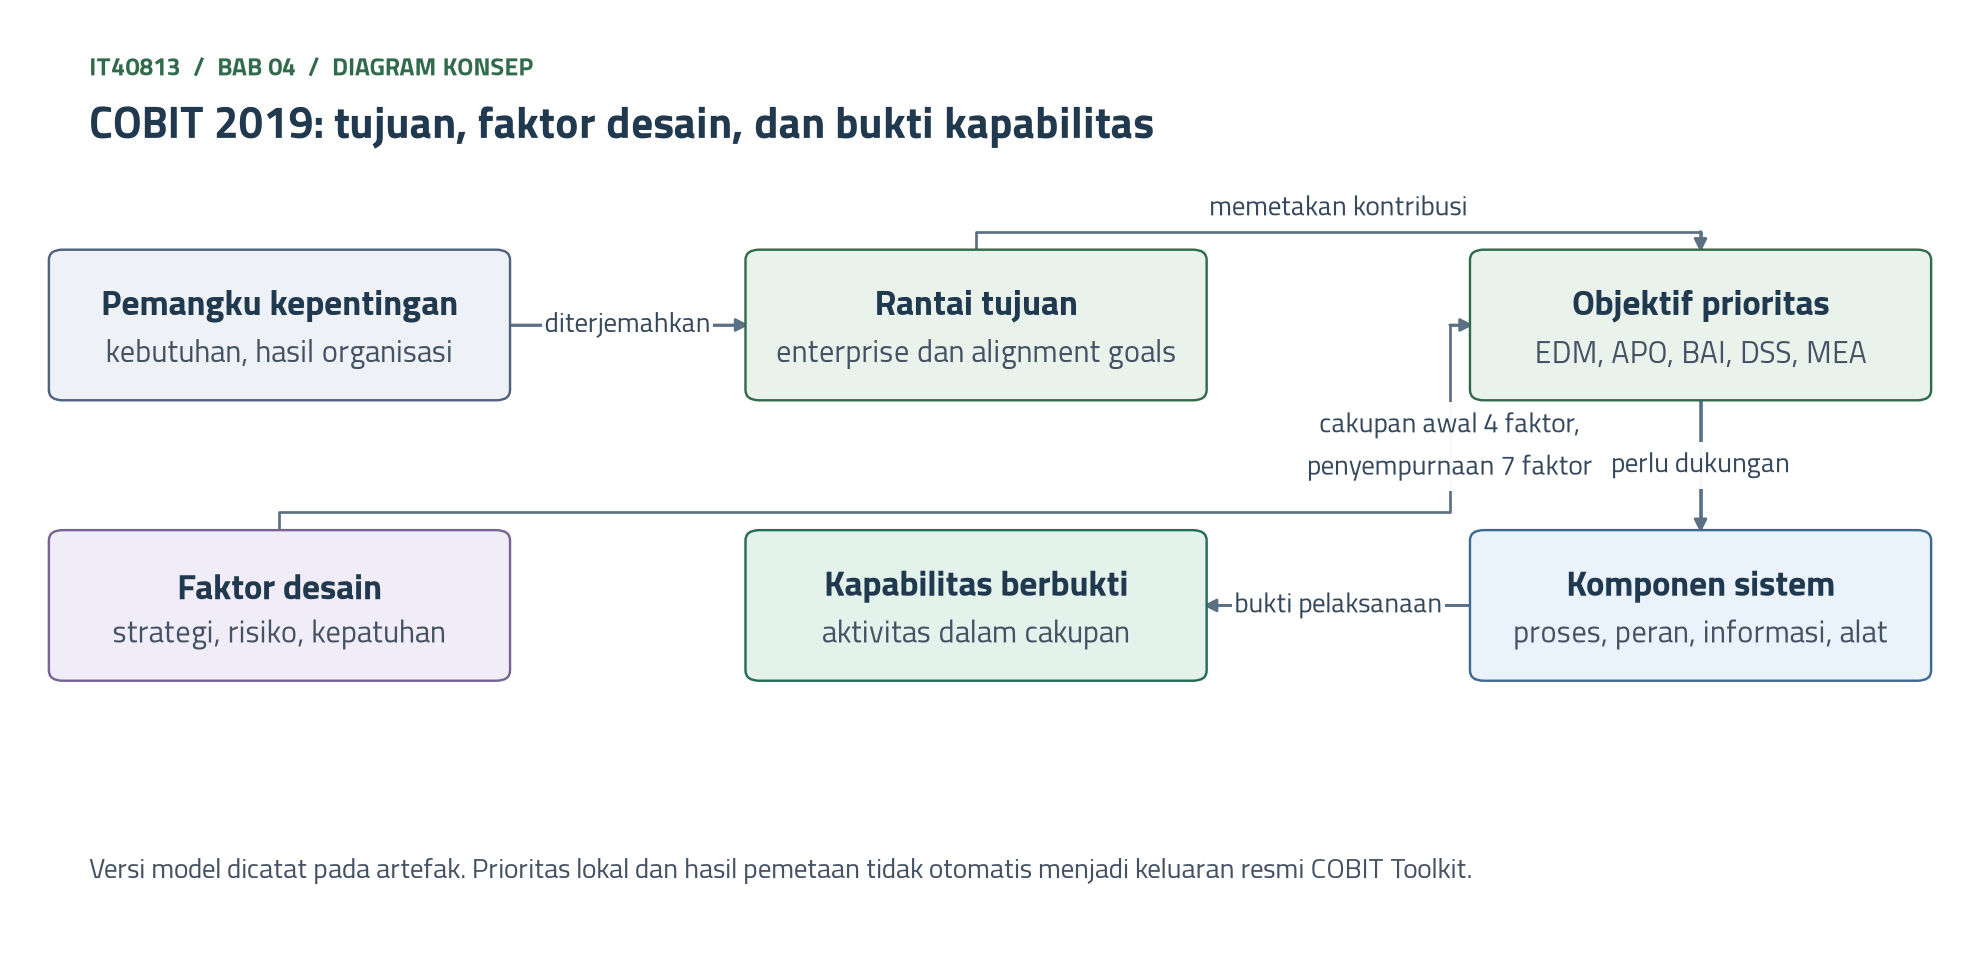
\includegraphics[width=0.96\textwidth,height=0.77\textheight,keepaspectratio]{../../figures/ch04-diagram-konsep.png}
  \label{fig:session04-ilustrasi-bab}
\end{frame}

\section{COBIT sebagai Kerangka}

\begin{frame}{{\Large Empat Publikasi Inti COBIT 2019}}
  \vspace{4pt}
  \footnotesize
  \begin{tabularx}{\textwidth}{|>{\raggedright\arraybackslash}p{0.38\textwidth}|>{\raggedright\arraybackslash}X|}
    \hline
    \textbf{Publikasi} & \textbf{Pertanyaan yang dijawab} \\ \hline
    Framework: Introduction and Methodology & Apa konsep dan prinsip kerangka ini? \\ \hline
    Framework: Governance and Management Objectives & Apa isi tiap objektif, praktik, dan aktivitasnya? \\ \hline
    Design Guide & Bagaimana merancang sistem sesuai konteks organisasi? \\ \hline
    Implementation Guide & Bagaimana menerapkan dan mengoptimalkan rancangan itu? \\ \hline
  \end{tabularx}

  \vspace{8pt}
  \small Isi COBIT bersifat umum dan perlu disesuaikan. Publikasi desain dan implementasi sudah menyatakan
  arah itu pada judulnya.
\end{frame}

\begin{frame}{{\Large Katalog Bukan Rencana Perbaikan}}
  \vspace{4pt}
  \small
  \begin{itemize}
    \item Analogi: bengkel punya katalog ratusan suku cadang, tetapi montir memilih bagian setelah memeriksa mobil.
    \item Kadam (2020): 4 objektif memuat 25 praktik dan 140 aktivitas, rata-rata 35 per objektif.
    \item Perkiraan kasar: 40 objektif sekitar 1.400 aktivitas. Dengan 30 menit per aktivitas: 700 jam, atau 87,5 hari kerja.
    \item Bab 1: 52 staf TI dibagi 40 objektif = 1,3 orang. Dibagi 6 objektif = sekitar 8,7 orang.
    \item Sertifikat 4 dari 52 staf (7,7 persen) tidak menjawab apakah 120 akun sudah ditinjau.
  \end{itemize}
\end{frame}

\begin{frame}{{\Large Kasus Medikara: Dari Perintah ke Tiga Pertanyaan}}
  \vspace{4pt}
  \small
  \begin{itemize}
    \item Masalah layanan mana yang paling merugikan? Siapa pemiliknya? Bukti apa yang diterima komite?
    \item Misalkan konsultan menawarkan Rp600 juta untuk 40 objektif.
    \item Rp600 juta melewati batas komite Rp400 juta, sehingga keputusan naik ke direksi.
    \item Bila biaya sebanding jumlah objektif, 6 objektif setara 15 persen, sekitar Rp90 juta.
    \item Rp90 juta di bawah batas Rp100 juta untuk kepala TI, dengan masukan pemilik layanan.
  \end{itemize}
\end{frame}

\section{Prinsip dan Komponen}

\begin{frame}{{\Large Enam Prinsip Sistem Tata Kelola}}
  \vspace{2pt}
  \scriptsize
  \begin{tabularx}{\textwidth}{|>{\raggedright\arraybackslash}p{0.3\textwidth}|>{\raggedright\arraybackslash}X|}
    \hline
    \textbf{Prinsip} & \textbf{Contoh pada Medikara (pengandaian)} \\ \hline
    Nilai bagi pemangku kepentingan & Ukuran utama: kerahasiaan data dan waktu tunggu, bukan jumlah prosedur \\ \hline
    Pendekatan menyeluruh & AC-01 memerlukan proses, daftar akun, pemilik, dan alat \\ \hline
    Sistem yang dinamis & Akuisisi fasilitas baru memicu penilaian ulang \\ \hline
    Tata kelola berbeda dari manajemen & Komite 9 anggota menilai arah; kepala TI menjalankan rencana \\ \hline
    Disesuaikan dengan kebutuhan & Medikara+ buatan vendor menaikkan perhatian pada vendor \\ \hline
    Mencakup seluruh fungsi & Cakupan 36 fasilitas, bukan hanya divisi TI pusat \\ \hline
  \end{tabularx}

  \vspace{6pt}
  \small Tiga prinsip kerangka: model konseptual; terbuka dan luwes; selaras dengan standar, kerangka, dan regulasi utama.
\end{frame}

\begin{frame}{{\Large Tujuh Komponen pada AC-01}}
  \vspace{2pt}
  \scriptsize
  \begin{tabularx}{\textwidth}{|>{\raggedright\arraybackslash}p{0.32\textwidth}|>{\raggedright\arraybackslash}X|>{\raggedright\arraybackslash}X|}
    \hline
    \textbf{Komponen} & \textbf{Penerapan AC-01} & \textbf{Bukti} \\ \hline
    Proses & Tarik daftar, tandai, cabut, catat & Catatan peninjauan bulanan \\ \hline
    Struktur organisasi & Pengelola vendor, pemilik layanan, eskalasi & Mandat dan daftar peran \\ \hline
    Prinsip, kebijakan, dan prosedur & Akun per orang, batas waktu pencabutan & Kebijakan akses yang disahkan \\ \hline
    Informasi & Populasi akun dan tanggal berakhir penugasan & Daftar 120 akun dan penugasan \\ \hline
    Budaya, etika, dan perilaku & Peninjau berani mencabut akses vendor penting & Tindak lanjut atas keberatan \\ \hline
    Orang, keterampilan, dan kompetensi & Peninjau memahami peran akses & Pelatihan dan hasil uji sampel \\ \hline
    Layanan, infrastruktur, dan aplikasi & Alat pencatatan serta pencabutan & Rekam perubahan akses \\ \hline
  \end{tabularx}
\end{frame}

\begin{frame}{{\Large Analogi dan Contoh Berangka}}
  \vspace{4pt}
  \small
  \begin{itemize}
    \item Perpustakaan butuh aturan, petugas, katalog, perangkat, dan kebiasaan mengembalikan. Prosedur saja tidak
          membuat buku kembali ke rak.
    \item Misalkan daftar yang diterima peninjau hanya memuat 108 dari 120 akun. Sebanyak 12 akun (10 persen) luput.
    \item Komponen yang lemah adalah informasi, jadi menambah prosedur tidak menutup celah.
    \item Misalkan 1 rumah sakit berbeda dari 4 lainnya karena SIMRS hasil akuisisi. Penyesuaian dijelaskan, bukan
          dinilai dari kesamaan format.
    \item Komite tidak mencabut 24 akun. Komite memastikan ada pemilik dan melihat hasilnya.
  \end{itemize}
\end{frame}

\section{Model Inti}

\begin{frame}{\hfill}
  \centering
  \Huge{\textbf{Model Inti:\\40 Objektif\\dalam Lima Domain}}
\end{frame}

\begin{frame}{{\Large Lima Domain dan Enam Objektif Awal}}
  \centering
  \vspace{2pt}
  \begin{tikzpicture}[
  kotak/.style={draw,rounded corners,align=center,text width=2.3cm,
    minimum height=1.6cm,font=\scriptsize,fill=blue!8},
  induk/.style={draw,rounded corners,align=center,text width=11.1cm,
    minimum height=0.95cm,font=\scriptsize,fill=praditagreen!15},
  pilih/.style={draw,rounded corners,align=center,text width=2.3cm,
    minimum height=0.95cm,font=\scriptsize,fill=orange!12},
  panah/.style={-{Stealth[length=2mm]},thick}
]
  \node[induk] (edm) at (4.35,2.35)
    {\textbf{EDM: 5 objektif tata kelola}\\
    {\tiny\mdseries mengevaluasi, mengarahkan, dan memantau}};
  \node[kotak] (apo) at (0,0)
    {\textbf{APO}\\14 objektif\\{\tiny\mdseries menyelaraskan dan merencanakan}};
  \node[kotak] (bai) at (2.9,0)
    {\textbf{BAI}\\11 objektif\\{\tiny\mdseries membangun dan memperoleh}};
  \node[kotak] (dss) at (5.8,0)
    {\textbf{DSS}\\6 objektif\\{\tiny\mdseries menjalankan dan mendukung}};
  \node[kotak] (mea) at (8.7,0)
    {\textbf{MEA}\\4 objektif\\{\tiny\mdseries memantau dan menilai}};
  \draw[panah] (apo) -- (bai);
  \draw[panah] (bai) -- (dss);
  \draw[panah] (dss) -- (mea);
  \draw[panah] (apo.north |- edm.south) -- node[right,font=\tiny] {arah} (apo.north);
  \draw[panah] (mea.north) -- node[left,font=\tiny] {laporan} (mea.north |- edm.south);
  \node[pilih] (p1) at (0,-1.5) {APO10, APO12, APO13, APO14};
  \node[pilih,fill=gray!35] (p2) at (2.9,-1.5) {BAI06 sebagai dependensi};
  \node[pilih] (p3) at (5.8,-1.5) {DSS05};
  \node[pilih] (p4) at (8.7,-1.5) {MEA03};
  \draw[thick,densely dashed] (apo) -- (p1);
  \draw[thick,densely dashed] (bai) -- (p2);
  \draw[thick,densely dashed] (dss) -- (p3);
  \draw[thick,densely dashed] (mea) -- (p4);
  \node[font=\scriptsize,align=center] at (4.35,-2.4)
    {5 + 14 + 11 + 6 + 4 = 40 objektif. Baris bawah: enam objektif awal pengandaian Medikara.};
\end{tikzpicture}

\end{frame}

\begin{frame}{{\Large Contoh Nama Objektif yang Sudah Dicocokkan}}
  \vspace{2pt}
  \scriptsize
  \begin{tabularx}{\textwidth}{|>{\raggedright\arraybackslash}p{0.11\textwidth}|>{\raggedright\arraybackslash}p{0.27\textwidth}|>{\raggedright\arraybackslash}X|}
    \hline
    \textbf{Domain} & \textbf{Fokus} & \textbf{Contoh objektif} \\ \hline
    EDM, 5 & Arah serta pengawasan & EDM03 \textit{Ensured risk optimization} \\ \hline
    APO, 14 & Perencanaan, pengorganisasian & APO10 \textit{Managed vendors}; APO12 \textit{Managed risk}; APO13 \textit{Managed security}; APO14 \textit{Managed data} \\ \hline
    BAI, 11 & Perolehan, perubahan solusi & BAI06 \textit{Managed IT changes}; BAI11 \textit{Managed projects} \\ \hline
    DSS, 6 & Operasi serta layanan & DSS04 \textit{Managed continuity}; DSS05 \textit{Managed security services} \\ \hline
    MEA, 4 & Pemantauan serta penilaian & MEA03 \textit{Managed compliance with external requirements}; MEA04 \textit{Managed assurance} \\ \hline
  \end{tabularx}

  \vspace{6pt}
  \small Katalog di \texttt{sources/chapter04}: 31 nama sudah dicocokkan, 9 ditandai ``perlu dicocokkan''.
\end{frame}

\begin{frame}{{\Large Objektif, Praktik, Aktivitas}}
  \vspace{4pt}
  \small
  \begin{itemize}
    \item Objektif menyatakan hasil. Isinya diuraikan menjadi praktik dan aktivitas. DSS04 memiliki 8 praktik.
    \item Tiap aktivitas dikaitkan dengan satu tingkat kapabilitas (Thomas, 2018).
    \item Analogi: peta layanan rumah sakit membagi unit, tetapi perjalanan satu pasien melewati beberapa unit.
    \item Misalkan temuan 6 dari 30 akun mengarah pada APO10 dan DSS05, yang dinilai bersama.
    \item Misalkan pembaruan aplikasi membuat 2.400 dari 96.000 data (2,5 persen) tidak cocok: BAI06 dan APO14.
  \end{itemize}
\end{frame}

\section{Faktor Desain}

\begin{frame}{\hfill}
  \centering
  \Huge{\textbf{Sebelas Faktor Desain\\dan Focus Area}}
\end{frame}

\begin{frame}{{\Large Faktor Dipakai Bertahap}}
  \centering
  \vspace{6pt}
  \begin{tikzpicture}[
  kotak/.style={draw,rounded corners,align=center,text width=2.5cm,
    minimum height=2.3cm,font=\scriptsize,fill=blue!8},
  panah/.style={-{Stealth[length=2mm]},thick}
]
  \node[kotak,fill=praditagreen!15] (a) at (0,0)
    {\textbf{Konteks}\\strategi dan keadaan organisasi\\
    {\tiny\mdseries sumber: dokumen dan wawancara}};
  \node[kotak] (b) at (3.0,0)
    {\textbf{Cakupan awal}\\4 faktor\\
    {\tiny\mdseries strategi, tujuan organisasi, profil risiko, isu TI}};
  \node[kotak,fill=orange!12] (c) at (6.0,0)
    {\textbf{Penyempurnaan}\\7 faktor\\
    {\tiny\mdseries ancaman, kepatuhan, peran TI, model penyediaan, metode implementasi,
    adopsi teknologi, ukuran}};
  \node[kotak,fill=green!10] (d) at (9.0,0)
    {\textbf{Kesimpulan}\\konflik diselesaikan\\
    {\tiny\mdseries objektif prioritas dan target kapabilitas}};
  \draw[panah] (a) -- (b);
  \draw[panah] (b) -- (c);
  \draw[panah] (c) -- (d);
  \draw[panah] (d.south) -- ++(0,-0.4) -| node[pos=0.25,below,font=\scriptsize]
    {faktor berubah: rancangan dinilai ulang} (a.south);
\end{tikzpicture}


  \vspace{8pt}
  \raggedright\small Empat faktor membuka cakupan awal, tujuh faktor memperhalus, lalu konflik diselesaikan. Analogi:
  jaringan air rumah satu lantai berbeda dari jaringan air rumah sakit.
\end{frame}

\begin{frame}{{\Large Sebelas Faktor pada Medikara}}
  \vspace{0pt}
  \footnotesize
  \begin{tabularx}{\textwidth}{|>{\raggedright\arraybackslash}p{0.27\textwidth}|>{\raggedright\arraybackslash}X|>{\raggedright\arraybackslash}p{0.17\textwidth}|}
    \hline
    \textbf{Faktor} & \textbf{Nilai pada Medikara} & \textbf{Status} \\ \hline
    Strategi organisasi & \textit{Client service/stability} tertinggi & Pengandaian \\ \hline
    Tujuan organisasi & EG06, EG03, EG12 & Pengandaian \\ \hline
    Profil risiko & \textit{Third-party/supplier incidents}; R-01 & Insiden: fakta \\ \hline
    Isu terkait TI & Temuan audit, layanan vendor, integrasi data & Fakta kasus \\ \hline
    Ancaman & \textit{High} 75 persen, \textit{normal} 25 persen & Pengandaian \\ \hline
    Kebutuhan kepatuhan & \textit{High}: K-01 sampai K-16 pada 36 fasilitas & Register C1 \\ \hline
    Peran TI & \textit{Factory} dan \textit{turnaround} & Pengandaian \\ \hline
    Model penyediaan & Medikara+ vendor; SIMRS \textit{on-premise} & Fakta kasus \\ \hline
    Metode implementasi & \textit{Traditional} 70, \textit{agile} 25, DevOps 5 persen & Pengandaian \\ \hline
    Strategi adopsi teknologi & \textit{Follower}: \textit{cloud} bertahap sampai 2030 & Pengandaian \\ \hline
    Ukuran organisasi & Sekitar 4.800 karyawan, 52 staf TI & Fakta kasus \\ \hline
  \end{tabularx}
\end{frame}

\begin{frame}{{\Large Konteks Mengubah Pilihan: Dua Rumah Sakit}}
  \vspace{4pt}
  \small
  \begin{itemize}
    \item Denpasar: 170 karyawan, 75 persen \textit{outsourcing}, lima objektif: APO12, APO13, BAI06, DSS04, DSS05.
    \item Kediri: DSS05, APO07, dan APO12. Hanya 2 objektif sama dari 6 yang berbeda.
    \item Studi pertama menyebut 11 faktor, studi kedua 10. Perbedaan metode perlu dicatat.
    \item Medikara: sekitar 4.800 karyawan, 19,2 kali batas 250 pada studi Denpasar. Klinik mitra 60 karyawan masuk rentang.
    \item Misalkan 36 fasilitas menjadi 38 (naik 5,6 persen). Tujuan sama, isu akses dinilai ulang.
  \end{itemize}
\end{frame}

\begin{frame}{{\Large Focus Area Bukan Domain Keenam}}
  \vspace{4pt}
  \small
  \begin{itemize}
    \item Faktor desain menggambarkan keadaan organisasi. \textit{Focus area} memberi perhatian pada satu tema.
    \item Panduan ISACA: DevOps, risiko informasi dan teknologi, keamanan informasi, organisasi kecil dan menengah.
    \item Analogi: klinik jantung tetap memakai laboratorium, farmasi, dan rekam medis yang sama.
    \item Misalkan tim platform 6 orang memakai panduan DevOps. Peninjauan 120 akun vendor tetap perlu dijawab.
    \item Misalkan klinik mitra punya 2 staf TI. Panduan organisasi kecil lebih masuk akal sebagai titik awal.
  \end{itemize}
\end{frame}

\section{Goals Cascade}

\begin{frame}{{\Large Rantai Tujuan: Contoh Kadam (2020)}}
  \centering
  \vspace{4pt}
  \begin{tikzpicture}[
  kotak/.style={draw,rounded corners,align=center,text width=3.3cm,
    minimum height=1.25cm,font=\scriptsize,fill=blue!8},
  saring/.style={draw,rounded corners,align=center,text width=2.3cm,
    minimum height=1.25cm,font=\scriptsize,fill=orange!12},
  panah/.style={-{Stealth[length=2mm]},thick}
]
  \node[kotak,fill=praditagreen!15] (k) at (0,0)
    {\textbf{Kebutuhan pemangku kepentingan}\\
    {\tiny\mdseries layanan tetap berjalan saat terganggu}};
  \node[kotak] (e) at (3.95,0)
    {\textbf{Tujuan organisasi}\\EG06\\
    {\tiny\mdseries \textit{business service continuity and availability}}};
  \node[kotak] (g) at (7.9,0)
    {\textbf{Tujuan keselarasan}\\AG07 primer\\
    {\tiny\mdseries AG02 dan AG05 sekunder}};
  \draw[panah] (k) -- (e);
  \draw[panah] (e) -- (g);
  \node[saring,fill=gray!35] (s0) at (-0.5,-2.25)
    {\textbf{40}\\{\tiny\mdseries objektif model inti}};
  \node[saring] (s1) at (2.45,-2.25)
    {\textbf{17}\\{\tiny\mdseries objektif berprioritas primer}};
  \node[saring] (s2) at (5.4,-2.25)
    {\textbf{8}\\{\tiny\mdseries daftar pendek sesuai konteks}};
  \node[saring,fill=green!10] (s3) at (8.35,-2.25)
    {\textbf{4}\\{\tiny\mdseries fokus awal: 25 praktik, 140 aktivitas}};
  \draw[panah] (s0) -- (s1);
  \draw[panah] (s1) -- (s2);
  \draw[panah] (s2) -- (s3);
  \draw[panah] (g.south) -- ++(0,-0.3) -| (s0.north);
\end{tikzpicture}


  \vspace{6pt}
  \raggedright\small COBIT 2019 memuat 13 EG dan 13 AG. Analogi: rencana perjalanan mulai dari tujuan, bukan kenyamanan kursi.
\end{frame}

\begin{frame}{{\Large Rantai Prioritas Medikara}}
  \vspace{2pt}
  \scriptsize
  \begin{tabularx}{\textwidth}{|>{\raggedright\arraybackslash}p{0.27\textwidth}|>{\raggedright\arraybackslash}p{0.09\textwidth}|>{\raggedright\arraybackslash}p{0.12\textwidth}|>{\raggedright\arraybackslash}p{0.13\textwidth}|>{\raggedright\arraybackslash}X|}
    \hline
    \textbf{Kebutuhan} & \textbf{EG} & \textbf{AG} & \textbf{Objektif} & \textbf{Status pemetaan} \\ \hline
    Kerahasiaan data pasien & EG06 & AG07 & APO13; DSS05 & Tercantum pada sumber \\ \hline
    Vendor dapat dipertanggungjawabkan & EG06 & AG05 & APO10 & Tercantum pada sumber \\ \hline
    Risiko layanan terkendali & EG02 & AG02 & APO12 & Penafsiran bab \\ \hline
    Identitas pasien konsisten & EG12 & AG08 & APO14 & Penafsiran bab \\ \hline
    Kewajiban dapat dibuktikan & EG03 & Belum ditetapkan & MEA03 & Penafsiran bab \\ \hline
  \end{tabularx}

  \vspace{6pt}
  \small Rafeq dan Elangovan (2021) memakai EG06 yang sama, tetapi memilih DSS04 dari enam objektif primer AG07.
  Alasan harus tertulis.
\end{frame}

\begin{frame}{{\Large Skor Lokal: Alat Diskusi, Bukan Keluaran Resmi}}
  \vspace{0pt}
  \footnotesize
  \begin{tabularx}{\textwidth}{|>{\raggedright\arraybackslash}p{0.12\textwidth}|>{\raggedright\arraybackslash}p{0.1\textwidth}|>{\raggedright\arraybackslash}p{0.14\textwidth}|>{\raggedright\arraybackslash}p{0.12\textwidth}|>{\raggedright\arraybackslash}p{0.08\textwidth}|>{\raggedright\arraybackslash}X|}
    \hline
    \textbf{Objektif} & \textbf{Risiko} & \textbf{Kewajiban} & \textbf{Strategi} & \textbf{Total} & \textbf{Keputusan} \\ \hline
    APO10 & 5 & 4 & 3 & 12 & Masuk \\ \hline
    DSS05 & 5 & 5 & 2 & 12 & Masuk \\ \hline
    APO13 & 4 & 4 & 3 & 11 & Masuk \\ \hline
    APO14 & 3 & 3 & 5 & 11 & Masuk \\ \hline
    APO12 & 4 & 3 & 3 & 10 & Masuk \\ \hline
    MEA03 & 2 & 5 & 3 & 10 & Masuk \\ \hline
    DSS04 & 3 & 4 & 3 & 10 & Ditunda ke Bab 10 \\ \hline
    BAI06 & 3 & 2 & 4 & 9 & Dependensi \\ \hline
    APO09 & 3 & 2 & 2 & 7 & Ditunda \\ \hline
  \end{tabularx}
\end{frame}

\begin{frame}{{\Large Kasus Medikara: Enam Objektif Awal}}
  \vspace{4pt}
  \small
  \begin{itemize}
    \item Misalkan pilihan: APO10, APO12, APO13, APO14, DSS05, dan MEA03. BAI06 sebagai dependensi.
    \item Tiga objektif bernilai 10, tersisa dua tempat. Alasan memutuskan: R-01 dan 16 baris register.
    \item DSS04 ditunda ke Bab 10, tetapi 36 prosedur dan 144 uji pemulihan per tahun tetap berjalan.
    \item Bila bobot kewajiban digandakan: APO12 turun ke urutan ketujuh, DSS04 masuk enam besar.
    \item Enam objektif setara 210 aktivitas atau 105 jam, jauh dari 700 jam untuk 40 objektif.
  \end{itemize}
\end{frame}

\section{Kapabilitas}

\begin{frame}{\hfill}
  \centering
  \Huge{\textbf{Kapabilitas:\\Bukti, Bukan Pengakuan}}
\end{frame}

\begin{frame}{{\Large Tingkat Kapabilitas 0 sampai 5}}
  \centering
  \vspace{6pt}
  \begin{tikzpicture}[
  anak/.style={draw,rounded corners,align=center,text width=1.68cm,
    minimum height=1.05cm,font=\scriptsize,fill=blue!8},
  panah/.style={-{Stealth[length=2mm]},thick}
]
  \node[anak,fill=gray!35] (t0) at (0,0)
    {\textbf{0}\\{\tiny\mdseries belum memadai}};
  \node[anak] (t1) at (1.95,0.8)
    {\textbf{1}\\{\tiny\mdseries aktivitas belum lengkap}};
  \node[anak] (t2) at (3.9,1.6)
    {\textbf{2}\\{\tiny\mdseries aktivitas dasar lengkap}};
  \node[anak,fill=orange!12] (t3) at (5.85,2.4)
    {\textbf{3}\\{\tiny\mdseries memakai aset organisasi}};
  \node[anak] (t4) at (7.8,3.2)
    {\textbf{4}\\{\tiny\mdseries kinerja diukur kuantitatif}};
  \node[anak,fill=green!10] (t5) at (9.75,4.0)
    {\textbf{5}\\{\tiny\mdseries perbaikan berkelanjutan}};
  \draw[panah] (t0.north) |- (t1.west);
  \draw[panah] (t1.north) |- (t2.west);
  \draw[panah] (t2.north) |- (t3.west);
  \draw[panah] (t3.north) |- (t4.west);
  \draw[panah] (t4.north) |- (t5.west);
  \node[font=\scriptsize,align=left,text width=6.6cm] at (6.75,0.3)
    {Tiap tingkat diperiksa lewat aktivitas dan buktinya pada cakupan yang tertulis.
    Tingkat yang lebih tinggi tidak otomatis menjadi target semua objektif.};
\end{tikzpicture}


  \vspace{6pt}
  \raggedright\small Skala mengacu pada CMMI. Skala COBIT 5 berbasis ISO/IEC 33000 tidak boleh dipindahkan begitu saja.
\end{frame}

\begin{frame}{{\Large Peringkat Capaian dan Aturan Penetapan}}
  \vspace{2pt}
  \footnotesize
  \begin{tabularx}{\textwidth}{|>{\raggedright\arraybackslash}p{0.27\textwidth}|>{\raggedright\arraybackslash}X|>{\raggedright\arraybackslash}X|}
    \hline
    \textbf{Peringkat} & \textbf{Souza Neto dan rekan} & \textbf{Studi Denpasar} \\ \hline
    N, \textit{not achieved} & Kurang dari 15 persen & 0 sampai 14 persen \\ \hline
    P, \textit{partially achieved} & 15 sampai 50 persen & 15 sampai 49 persen \\ \hline
    L, \textit{largely achieved} & 50 sampai 85 persen & 50 sampai 84 persen \\ \hline
    F, \textit{fully achieved} & Lebih dari 85 persen & 85 sampai 100 persen \\ \hline
  \end{tabularx}

  \vspace{4pt}
  \small
  \begin{itemize}
    \item Dua studi rumah sakit: satu tingkat tercapai bila capaian penuh. Denpasar: 85 persen atau lebih.
    \item Kediri: APO07 80,55 persen pada tingkat 2, peringkat L, tetap tingkat 1.
    \item Aturan perlu ditulis dan dicocokkan ke publikasi ISACA sebelum asesmen formal.
  \end{itemize}
\end{frame}

\begin{frame}{{\Large Membaca Dua Studi Secara Kritis}}
  \vspace{2pt}
  \scriptsize
  \begin{tabularx}{\textwidth}{|>{\raggedright\arraybackslash}p{0.2\textwidth}|>{\raggedright\arraybackslash}X|>{\raggedright\arraybackslash}X|}
    \hline
    \textbf{Aspek} & \textbf{Rumah Sakit Umum Bhakti Rahayu} & \textbf{Rumah Sakit Wilujeng} \\ \hline
    Tingkat saat ini & APO12, DSS04: 1; APO13, BAI06, DSS05: 2 & DSS05, APO07, APO12: 1 \\ \hline
    Sumber data & Kuesioner 5 karyawan, observasi, wawancara & Kuesioner, manajer unit TI, 1 responden sumber daya manusia \\ \hline
    Pertanyaan pembaca & Bukti apa yang menopang jawaban? & Apakah satu manajer menilai pekerjaannya sendiri? \\ \hline
  \end{tabularx}

  \vspace{4pt}
  \small
  \begin{itemize}
    \item Denpasar, APO12: 66, 66, 50, 50, 83 persen, rata-rata 63. Selisih 33 poin tersembunyi.
    \item Denpasar, APO13: kelima responden 71 persen. Lima pengamatan atau satu pendapat?
    \item Foto dapur bersih tidak membuktikan kebersihan sepanjang bulan.
  \end{itemize}
\end{frame}

\begin{frame}{{\Large Bukti dan Batas Klaim}}
  \vspace{4pt}
  \footnotesize
  \begin{tabularx}{\textwidth}{|>{\raggedright\arraybackslash}p{0.26\textwidth}|>{\raggedright\arraybackslash}X|>{\raggedright\arraybackslash}X|}
    \hline
    \textbf{Klaim} & \textbf{Bukti yang diperlukan} & \textbf{Batas kesimpulan} \\ \hline
    Pekerjaan dilakukan & Contoh hasil dan pelaksana & Belum membuktikan konsistensi \\ \hline
    Cara kerja terdefinisi & Prosedur, penerapan lintas unit & Perlu sampel beberapa periode \\ \hline
    Kinerja diukur & Definisi metrik dan data andal & Angka tanpa tindakan belum cukup \\ \hline
    Perbaikan berkelanjutan & Analisis, tindakan, hasil ulang & Perlu keterkaitan sebab dan hasil \\ \hline
  \end{tabularx}

  \vspace{8pt}
  \small Misalkan 8 dari 10 perubahan punya persetujuan, tetapi 2 perubahan darurat tanpa analisis dampak. Yang gagal justru
  jenis paling berisiko.
\end{frame}

\begin{frame}{{\Large Kasus Medikara: Potret Cepat DSS05 Lewat AC-01}}
  \vspace{4pt}
  \small
  \begin{itemize}
    \item Audit: 6 dari 30 akun masih aktif. Peninjauan penuh: 24 dari 120 dicabut. Keduanya 20 persen.
    \item Sampel hanya satu lokasi, sehingga tidak diproyeksikan. Pada sampel, 24 dari 30 akun (80 persen) sesuai, peringkat \textit{largely}.
    \item Bukti peninjauan hanya ada di 1 dari 5 rumah sakit.
    \item Kesimpulan: tingkat indikatif 1 untuk satu rumah sakit. Klaim lintas 5 rumah sakit ditolak sementara.
    \item AC-01 hanya satu bagian DSS05, jadi hasil ini bukan tingkat DSS05 keseluruhan.
  \end{itemize}
\end{frame}

\section{Kaitan dan Versi}

\begin{frame}{{\Large Kaitan dengan ITIL 4 dan Tata Kelola Arsitektur}}
  \vspace{2pt}
  \scriptsize
  \begin{tabularx}{\textwidth}{|>{\raggedright\arraybackslash}p{0.13\textwidth}|>{\raggedright\arraybackslash}X|>{\raggedright\arraybackslash}X|>{\raggedright\arraybackslash}X|}
    \hline
    \textbf{Aspek} & \textbf{COBIT 2019} & \textbf{ITIL 4} & \textbf{Tata kelola arsitektur} \\ \hline
    Pertanyaan & Hasil apa yang dicapai dan dibuktikan? & Bagaimana layanan dijalankan sehari-hari? & Susunan mana dipilih, siapa memutuskan? \\ \hline
    Contoh & BAI06 perubahan TI & \textit{Change enablement} & Keputusan pola integrasi \\ \hline
    Bukti & Tingkat kapabilitas dan celah & Tiket dan jadwal perubahan & Catatan keputusan arsitektur \\ \hline
    Dibahas di & Bab ini & Bab 8 & IT40513 \\ \hline
  \end{tabularx}

  \vspace{6pt}
  \small
  \begin{itemize}
    \item Misalkan 10 tiket perubahan: satu bukti terbaca oleh dua kerangka.
    \item Integrasi Rp450 juta, toleransi 10 persen, batas Rp495 juta: forum arsitektur memutuskan pola, COBIT memeriksa pemilik dan bukti.
  \end{itemize}
\end{frame}

\begin{frame}{{\Large Transisi ke COBIT 7}}
  \vspace{2pt}
  \footnotesize
  \begin{tabularx}{\textwidth}{|>{\raggedright\arraybackslash}p{0.22\textwidth}|>{\raggedright\arraybackslash}X|}
    \hline
    \textbf{Tanggal} & \textbf{Peristiwa (pengumuman ISACA Sydney Chapter)} \\ \hline
    26 Oktober 2026 & Batas pembelian sertifikat COBIT 2019 \\ \hline
    27 Oktober & Debut COBIT 7 dan sertifikat Foundation \\ \hline
    26 April 2027 & Batas ujian COBIT 2019, sisa 177 hari dari 31 Oktober 2026 \\ \hline
  \end{tabularx}

  \vspace{4pt}
  \small
  \begin{itemize}
    \item Pada 31 Oktober 2026, halaman sumber daya COBIT yang terbaca masih menampilkan COBIT 2019.
    \item Teks resmi COBIT 7 belum diperoleh, jadi modul memakai model COBIT 2019.
    \item Perubahan pengenal tidak boleh disimpulkan dari pengumuman saja.
  \end{itemize}
\end{frame}

\begin{frame}{{\Large Pemeriksaan Saat Mengganti Versi}}
  \vspace{4pt}
  \footnotesize
  \begin{tabularx}{\textwidth}{|>{\raggedright\arraybackslash}p{0.22\textwidth}|>{\raggedright\arraybackslash}X|>{\raggedright\arraybackslash}X|}
    \hline
    \textbf{Langkah} & \textbf{Hasil yang disimpan} & \textbf{Risiko bila dilewati} \\ \hline
    Tetapkan versi & Identitas model dan tanggal & Definisi bercampur \\ \hline
    Petakan perubahan & Hubungan unsur lama dan baru & Angka tidak sebanding \\ \hline
    Uji contoh & Penilaian ulang satu proses & Perbedaan penilai tersembunyi \\ \hline
    Setujui transisi & Keputusan serta jadwal & Artefak tidak sinkron \\ \hline
  \end{tabularx}

  \vspace{8pt}
  \small Preseden: COBIT 5 punya 37 proses, COBIT 2019 punya 40. Lembar kerja lama tidak punya baris untuk APO14, BAI11,
  dan MEA04.
\end{frame}

\section{Aktivitas dan Penutup}

\begin{frame}{{\Large Aktivitas: Alur dan Pembagian Peran}}
  \centering
  \vspace{2pt}
  \begin{tikzpicture}[
  kotak/.style={draw,rounded corners,align=center,text width=2.35cm,
    minimum height=1.25cm,font=\scriptsize,fill=blue!8},
  panah/.style={-{Stealth[length=2mm]},thick}
]
  \node[kotak,fill=praditagreen!15] (a) at (0,0) {Konteks, faktor desain, dan tujuan};
  \node[kotak,fill=orange!12] (b) at (3.05,0) {Objektif prioritas serta alasan};
  \node[kotak] (c) at (6.1,0) {Bukti kapabilitas dan celah};
  \node[kotak,fill=green!10] (d) at (9.15,0) {Masukan C2 untuk risiko Bab 5 dan target Bab 8};
  \draw[panah] (a) -- (b);
  \draw[panah] (b) -- (c);
  \draw[panah] (c) -- (d);
  \draw[panah] (c.south) -- ++(0,-0.45) -| node[pos=0.25,below,font=\scriptsize]
    {bukti baru dapat mengubah prioritas} (a.south);
\end{tikzpicture}


  \vspace{4pt}
  \raggedright\small
  \begin{itemize}
    \item Pemilik konteks mengumpulkan notulen, prosedur, dan hasil kerja.
    \item Analis risiko mengisi risiko dan ancaman. Analis regulasi mengisi kepatuhan.
    \item Analis teknologi mengisi peran TI, penyediaan, dan metode implementasi.
  \end{itemize}
\end{frame}

\begin{frame}{{\Large Aktivitas: Langkah Kerja}}
  \vspace{4pt}
  \small
  \begin{itemize}
    \item Isi sebelas faktor desain beserta sumber bukti dan asumsi.
    \item Turunkan sedikitnya tiga kebutuhan menjadi EG dan AG. Tandai sumber atau penafsiran.
    \item Beri skor kandidat, tulis bobot, ubah satu bobot, lalu pilih lima sampai tujuh objektif.
    \item Untuk tiap objektif, tentukan aktivitas, periode, populasi, dan sampel. Nilai berpasangan.
    \item Bandingkan dengan matriks keputusan C1 dan register kewajiban, lalu susun bukti tambahan.
  \end{itemize}
\end{frame}

\begin{frame}{{\Large Aktivitas: Luaran C2 dan Kriteria}}
  \vspace{4pt}
  \small
  \begin{itemize}
    \item Luaran: lembar faktor desain, rantai tujuan, skor lokal, objektif prioritas, potret kapabilitas.
    \item Masuk C2 Kondisi Saat Ini. Celah diteruskan ke risiko Bab 5 dan target Bab 8.
    \item Kriteria: konteks 25 persen; keterlacakan 30 persen; mutu bukti 30 persen; rekomendasi 15 persen.
    \item Berkas: \texttt{sources/chapter04/}, lima lembar kerja dengan \texttt{README.md}.
    \item Data organisasi nyata wajib berizin dan dianonimkan. Data pribadi tidak boleh dipakai.
  \end{itemize}
\end{frame}

\begin{frame}{{\Large Ringkasan}}
  \vspace{4pt}
  \small
  \begin{itemize}
    \item Enam prinsip dan tujuh komponen: prosedur saja tidak membuat proses berjalan.
    \item Empat puluh objektif memberi bahasa bersama. Lingkup adalah keputusan yang dipertanggungjawabkan.
    \item Sebelas faktor desain dan rantai tujuan memilih prioritas. Skor lokal berguna bila bobot tertulis.
    \item Kapabilitas dinilai lewat aktivitas dan bukti dalam lingkup yang jelas.
    \item Prioritas yang dapat dijelaskan dan bukti yang dapat diperiksa lebih berguna daripada mengejar seluruh kerangka.
  \end{itemize}
\end{frame}

\begin{frame}{{\Large Latihan dan Bacaan}}
  \vspace{2pt}
  \footnotesize
  \begin{enumerate}
    \item Dua rumah sakit memiliki strategi yang sama, tetapi satu mengembangkan sistem sendiri dan satu bergantung pada
          vendor. Bagaimana perbedaan model \textit{sourcing} itu menggeser objektif prioritas?
    \item Seorang manajer menyatakan proses manajemen perubahan sudah berada di tingkat kapabilitas 3. Bukti apa yang perlu
          diminta untuk menguji klaim itu?
    \item Jelaskan mengapa COBIT tidak dimaksudkan untuk diterapkan seluruhnya sekaligus.
  \end{enumerate}
  \vspace{4pt}
  \textbf{Bacaan:} \href{https://www.isaca.org/resources/cobit}{COBIT 2019};
  \href{https://www.isaca.org/resources/news-and-trends/industry-news/2020/evaluating-business-service-continuity-and-availability-using-cobit-2019}{Kadam (2020)};
  \href{https://www.isaca.org/resources/news-and-trends/industry-news/2019/defining-target-capability-levels-in-cobit-2019-a-proposal-for-refinement}{Souza Neto dan rekan (2019)};
  \href{https://doi.org/10.36040/jati.v9i3.13540}{Sari dan rekan (2025)}.
\end{frame}

\end{document}
